\documentclass{book}

\newcommand{\vcsbeam}{{\sc VCSBeam}}

\title{\vcsbeam{} Documentation}
\author{Dr. Sammy McSweeney}

\usepackage{amsmath}
\usepackage{fullpage}
\usepackage{listings}
\usepackage{graphicx}
\usepackage{hyperref}
\usepackage{natbib}
\usepackage{makeidx}

\setcounter{secnumdepth}{4}
\setcounter{tocdepth}{4}

\hypersetup{
    colorlinks=true,
    linkcolor=blue,
    filecolor=blue,
}

\makeindex

\newcommand{\pd}[2]{\ensuremath{\frac{\partial #1}{\partial #2}}}
\newcommand{\transmat}[4]{\ensuremath{{\bf P}_{(#1,#2)\rightarrow(#3,#4)}}}
\newcommand{\pamat}{\ensuremath{{\bf P}_\text{pa}}}

\begin{document}

\maketitle

\tableofcontents

\chapter{Conventions}

\section{Coordinate systems}

There are three coordinate systems in use throughout \vcsbeam{}:
\begin{enumerate}
    \item Instrumental ($p$,$q$)
    \item Local sky coordinates ($\theta$,$\phi$)
    \item Celestial sky coordinates ($x$,$y$)
\end{enumerate}
They are illustrated in Fig. \ref{fig:coords}.
\begin{figure}[!bh]
    \centering
    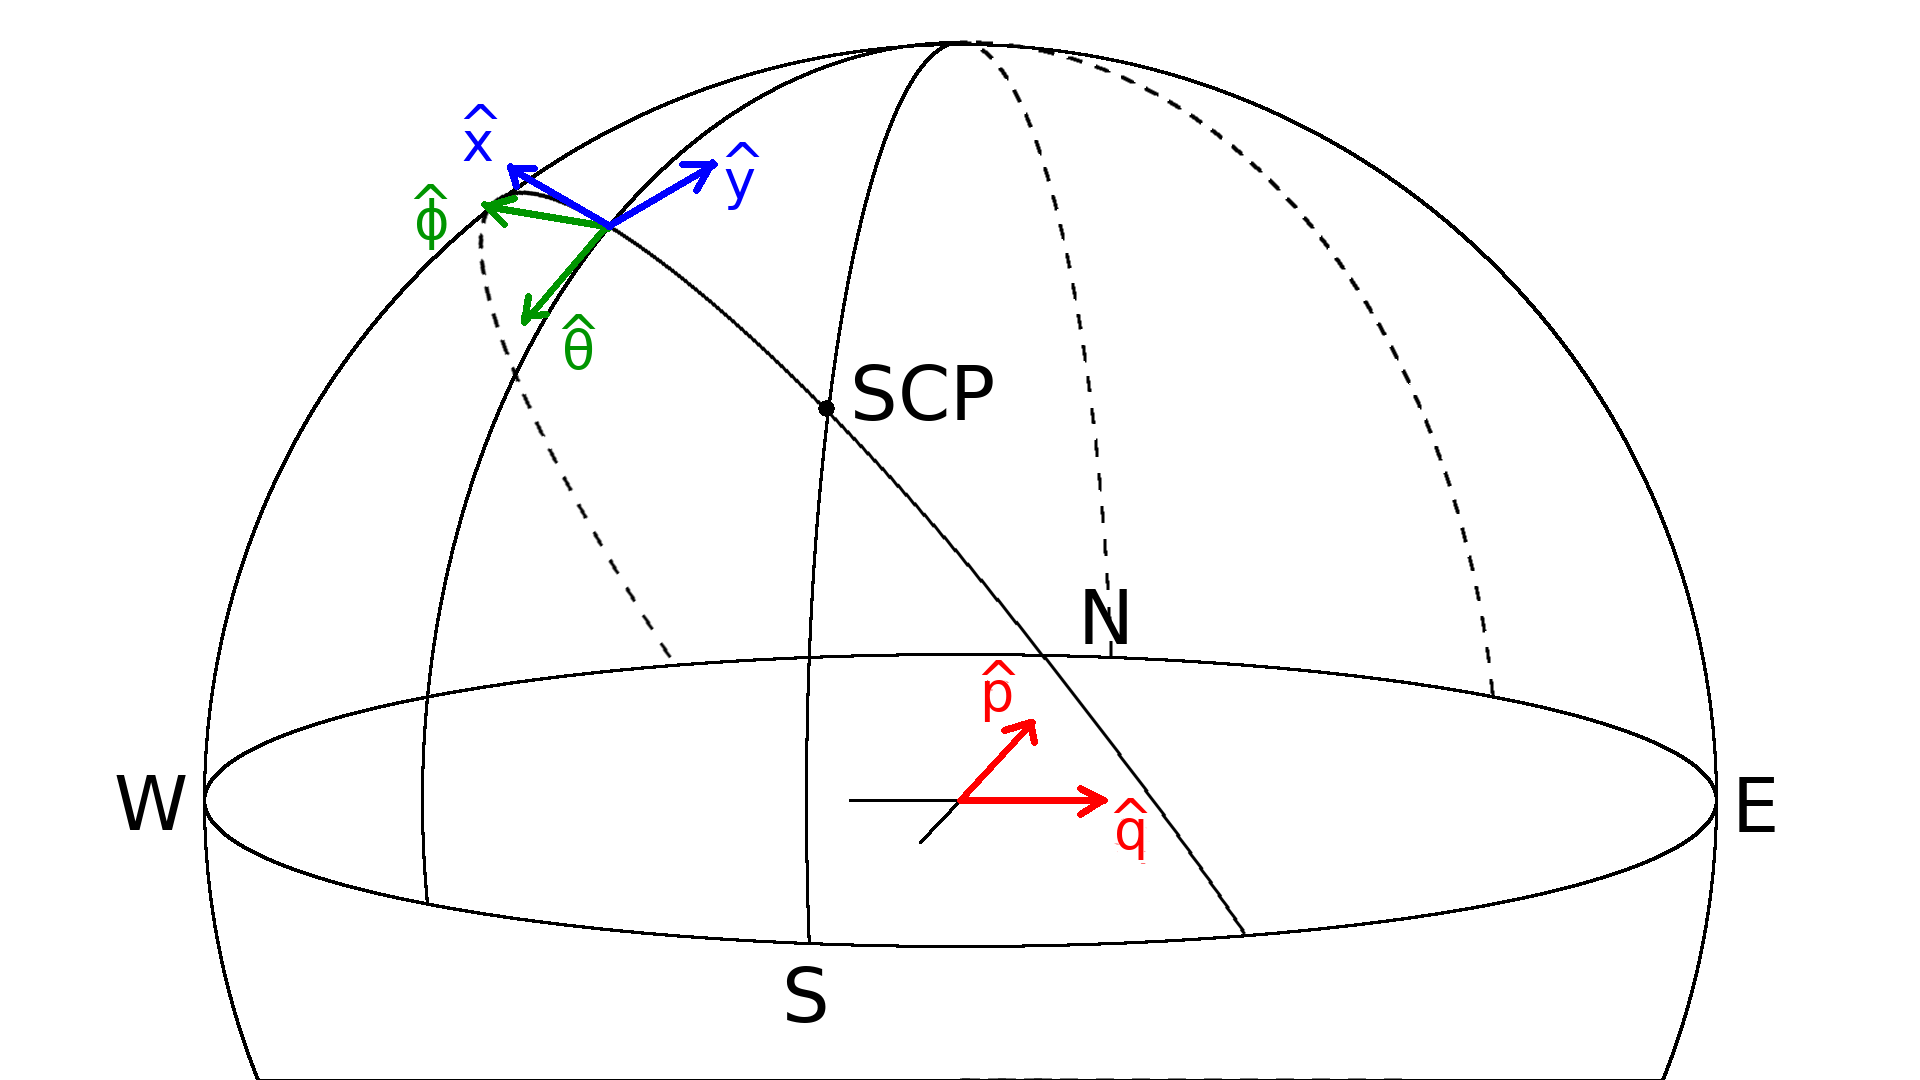
\includegraphics[width=\textwidth]{coords.png}
    \caption{Illustration of the three coordinate systems used in this work\dots}
    \label{fig:coords}
\end{figure}

\subsection{Instrumental coordinates}
\index{coordinates!instrumental}

This is a Cartesian coordinate system aligned with local (ground) compass directions.
Positive $p$ points towards local North, and positive $q$ towards local East.
The ``$P$ polarisation'' refers to the physical set of dipoles parallel to the N-S line; the ``$Q$ polarisation'', to the E-W line.

\subsection{Local sky coordinates}
\label{sec:coordslocalsky}
\index{coordinates!local sky}

This is a spherical coordinate system defined with respect to a local observer.
$\theta$ is the \textit{zenith angle}\index{zenith angle}, i.e. a \textit{colatitude}, with zenith itself therefore defined as $\theta = 0$ and the horizon as $\theta = \pi/2$.
$\phi$ is the \textit{azimuth}\index{azimuth}, and we define $\phi = 0$ in the North direction, with positive azimuth moving clockwise as viewed from above (i.e. N$\rightarrow$E$\rightarrow$S$\rightarrow$W$\rightarrow$N).
Moreover, the \textit{elevation}\index{elevation} is denoted by the symbol $\tilde{\theta}$, and is related to the zenith angle by
\begin{equation}
    \tilde{\theta} = \frac{\pi}{2} - \theta.
\end{equation}

\subsection{Celestial sky coordinates}
\index{coordinates!celestial sky}

This is a spherical coordinate system defined with respect to the celestial sphere.
$x$ is the \textit{declination}\index{declination} (Dec) and $y$ is the \textit{right ascension}\index{right ascension} (RA).

\subsection{Comparison of notation in other documents}

See Table \ref{tbl:notations}
\begin{table}[!hb]
    \centering
    \caption{Comparison of notation used elsewhere}
    \label{tbl:notations}
    \begin{tabular}{l|cc|cc|cc}
        & $p$ & $q$ & $\theta$ & $\phi$ & $x$ & $y$ \\
        \hline
        MWA metafits files       & Y & X & - & - & - & - \\
        Sokolowksi et al. (2017) & $y$ & $x$ & $\theta$ & $\phi$ & - & - \\
    \end{tabular}
\end{table}

\subsection{Coordinate transformations}

All coordinate transformations can be effected by applying the appropriate Jacobian matrix for the desired transformation.
In this work, a boldface ${\bf P}$ will always be used\footnote{``${\bf J}$'' is reserved for (other) Jones matrices.} to denote such transformation matrices.
For general coordinates $(a,b)$ and $(c,d)$,
\begin{equation}
    \transmat{a}{b}{c}{d} =
    \begin{bmatrix}
        \pd{c}{a} & \pd{c}{b} \\[5 pt]
        \pd{d}{a} & \pd{d}{b}
    \end{bmatrix}
\end{equation}
The specific transformations relevant to this work are specified in the following sections.

\subsubsection{Parallactic angle correction}

The parallactic angle correction is a transformation between local sky coordinates and celestial sky coordinates.
The parallactic angle itself, $\chi$, is defined as the position angle of local zenith with respect to the North Celestial Pole as subtended at a given source (see Fig. \ref{fig:skyangles}).
The transformation $(x,y)\rightarrow(\theta,\phi)$ is therefore a clockwise rotation\footnote{A counterclockwise rotation of a given vector is equivalent to a clockwise rotation of the coordinate axes.} by $\pi - \chi$.
This is the rotation
\begin{equation}
    \transmat{\theta}{\phi}{x}{y}
        = \begin{bmatrix}
             \cos\left(\pi - \chi\right) & \sin\left(\pi - \chi\right) \\
            -\sin\left(\pi - \chi\right) & \cos\left(\pi - \chi\right)
        \end{bmatrix}
        = \begin{bmatrix}
            -\cos\chi &  \sin\chi \\
            -\sin\chi & -\cos\chi
        \end{bmatrix}.
\end{equation}
\begin{figure}[!th]
    \centering
    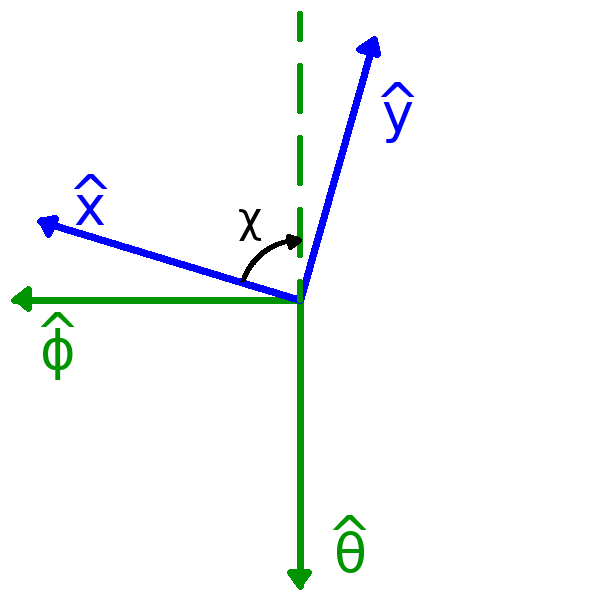
\includegraphics[width=0.4\textwidth]{skyangles.png}
    \caption{Definition of the parallactic angle, $\chi$, in the sky plane.}
    \label{fig:skyangles}
\end{figure}
The actual parallactic angle correction that is implemented is for historical reasons the matrix
\begin{equation}
    \pamat \equiv
    \transmat{\theta}{\phi}{y}{x}
        = \begin{bmatrix} 0 & 1 \\ 1 & 0 \end{bmatrix} \transmat{\theta}{\phi}{x}{y}
        = \begin{bmatrix}
             \sin\chi & -\cos\chi \\
            -\cos\chi & -\sin\chi
        \end{bmatrix}.
\end{equation}
In \vcsbeam{}, the parallactic angle is calculated (via the function \texttt{palPa} in the \href{https://github.com/Starlink/pal}{Starlink/pal} library) via the spherical triangle identity
\begin{equation}
    \tan \chi = \frac{\cos \lambda \sin H}{\sin\lambda \cos x - \cos \lambda \sin x \cos H},
\end{equation}
where $\lambda$ is the latitude of the observer\footnote{The latitude of the MWA is $\lambda_\text{MWA} = -0.4660608448386394\,$rad, defined in the \texttt{mwalib} library.}, $H$ is the hour angle of the source, and $x$ is the declination.

\chapter{Algorithms}

\section{PFB}

\subsection{Fine channelisation}

\section{Calibration}

\subsection{RTS}

\section{Beamforming}

\section{Applications}

\section{Utilities}

\chapter{Implementation}

\section{Code glossary}

\subsection{\texttt{az}}
\begin{description}
    \item[Name:] \hyperlink{sec:coordslocalsky}{Geographic azimuth}\index{azimuth!geographic}
    \item[Units:] radians
    \item[Functions:] \hyperlink{cn:calc_beam_geom}{\texttt{calc\_beam\_geom}}
\end{description}

\subsection{\texttt{el}}
\begin{description}
    \item[Name:] \hyperlink{sec:coordslocalsky}{Elevation}\index{elevation}
    \item[Units:] radians
    \item[Functions:] \hyperlink{cn:calc_beam_geom}{\texttt{calc\_beam\_geom}}
\end{description}

\subsection{\texttt{za}}
\begin{description}
    \item[Name:] \hyperlink{sec:coordslocalsky}{Zenith angle}\index{zenith angle}
    \item[Units:] radians
    \item[Functions:] \hyperlink{cn:calc_beam_geom}{\texttt{calc\_beam\_geom}}
\end{description}

\section{Function reference}

\subsection{\texttt{calc\_beam\_geom}}
\label{fcn:calc_beam_geom}

\printindex

\end{document}
